\documentclass[11pt]{standalone}
\usepackage{amssymb}
\usepackage{amsmath}
\usepackage[no-math]{fontspec}
\usepackage{unicode-math}
\usepackage{libertinus}
\usepackage{pgf,xcolor}
\usepackage{tikz}
\usetikzlibrary{arrows.meta, backgrounds}
\usepackage{pgfplots}
\pgfplotsset{compat=newest}

\definecolor{my_darkgray}{HTML}{484949}
\definecolor{my_lightgray}{HTML}{F3F4F4}
\definecolor{my_darkblue}{HTML}{005A94}
\definecolor{my_lightblue}{HTML}{CCDEE9}
\definecolor{my_yellow}{HTML}{FFEC7F}
\definecolor{my_red}{HTML}{E60000}
\definecolor{my_orange}{HTML}{E87846}

\begin{document}
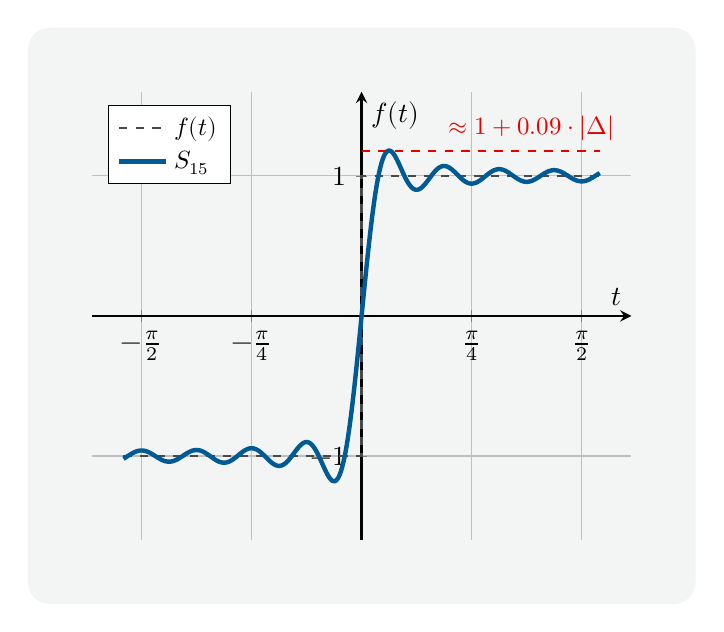
\begin{tikzpicture}[
    show background rectangle,
    background rectangle/.style={fill=my_lightgray, rounded corners=8pt},
    inner frame sep=0.8cm
]
\begin{axis}[
    axis lines = center,
    xlabel = {$t$},
    ylabel = {$f(t)$},
    grid = both,
    axis equal,
    axis line style={thick},
    xmin=-1.7, xmax=1.7,
    ymin=-1.6, ymax=1.6,
    xtick={-1.5708, -0.7854, 0, 0.7854, 1.5708},
    xticklabels={$-\tfrac{\pi}{2}$, $-\tfrac{\pi}{4}$, $0$,
                 $\tfrac{\pi}{4}$, $\tfrac{\pi}{2}$},
    ytick={-1, 1},
    yticklabels={$-1$, $1$},
    legend pos=north west,
    legend style={font=\small},
    legend cell align=left,
]
% Rechteck-Lagerkraft als Referenz (gestrichelt, sekundaer):
% Sprung von -1 auf +1 bei t = 0
\addplot[draw=my_darkgray, thick, dashed] coordinates {
    (-1.7, -1)
    (0, -1)
    (0, 1)
    (1.7, 1)
};
\addlegendentry{$f(t)$}
% Partialsumme S_15 der Rechteckschwingung:
% (4/pi) * Summe sin(n t)/n ueber ungerade n = 1, 3, ..., 15
\addplot[draw=my_darkblue, samples=400, ultra thick, domain=-1.7:1.7]
    {(4/pi)*( sin(deg(x))
            + sin(3*deg(x))/3
            + sin(5*deg(x))/5
            + sin(7*deg(x))/7
            + sin(9*deg(x))/9
            + sin(11*deg(x))/11
            + sin(13*deg(x))/13
            + sin(15*deg(x))/15 )};
\addlegendentry{$S_{15}$}
% Markierung des Gibbs-Ueberschwingers: ca. 1.179 = 1 + 0.09 * Sprunghoehe 2
\addplot[draw=my_red, semithick, dashed, domain=0:1.7] {1.179};
\node[anchor=south west, font=\small, color=my_red]
    at (axis cs:0.55, 1.18) {$\approx 1 + 0.09\cdot|\Delta|$};
\end{axis}
\end{tikzpicture}
\end{document}
